\documentclass{article}

\usepackage{polski}
\usepackage[utf8]{inputenc}
\usepackage{graphicx}
\usepackage{amsfonts}
\usepackage{amssymb}
\usepackage{amsmath}
\usepackage{listings}
\usepackage{breqn}
\usepackage{float}

\author{Maciej Pieta \and Piotr Koproń \and Jakub Woś \and Rafał Piwowar}
\date{Marzec 2023}

\title{Technika Cyfrowa. \\ Ćwiczenie 1.}

\begin{document}
\maketitle
\newpage
\section{Zadanie 1a}
\subsection{Treść zadania}
\paragraph{}
Bazując wyłącznie na dwuwejściowych bramkach logicznych NAND, proszę od podstaw  zaprojektować, zbudować i przetestować układ realizujący funkcję logiczną:
\begin{equation}
Y = \overline{A} \text{ xor } (B + C)
\end{equation}
\subsection{Rozwiązanie teoretyczne}
Dokonujemy następujących przekształceń, korzystając z definicji xor, praw de Morgana oraz prawa podwójnej negacji.
\begin{align*}
 Y &= \overline{A} \text{ xor } (B + C) \\
 &= \overline{A} \cdot \overline{(B+C)} + \overline{\overline{A}} \cdot (B+C)\\
&= \overline{A} \cdot (\overline{B} \cdot \overline{C}) + A \cdot (B+C)\\
&= \overline{A} \cdot \overline{\overline{(\overline{B} \cdot \overline{C})}} + A \cdot \overline{\overline{(B+C)}} \\
&= \overline{A} \cdot \overline{\overline{(\overline{B} \cdot \overline{C})}} + A \cdot \overline{(\overline{B} \cdot \overline{C})} \\
|K = \overline{(\overline{B} \cdot \overline{C})}| &= \overline{A} \cdot \overline{K} + A \cdot K \\
&= \overline{\overline{\overline{A} \cdot \overline{K} + A \cdot K}} \\
&= \overline{\overline{\overline{A} \cdot \overline{K}} \cdot \overline{A \cdot K}} \\
&= \overline{\overline{\overline{A} \cdot \overline{\overline{(\overline{B} \cdot \overline{C})}}} \cdot \overline{A \cdot \overline{(\overline{B} \cdot \overline{C})}}}
\end{align*}
Otrzymaliśmy równoważny układ bezpośrednio zapisujący się jako zbiór bramek NAND, przy obserwacji, że $x$ NAND 1 = $\overline{x}$.
\newpage
\subsection{Implementacja układu 1a w programie Multisim}
\begin{figure}[h!]
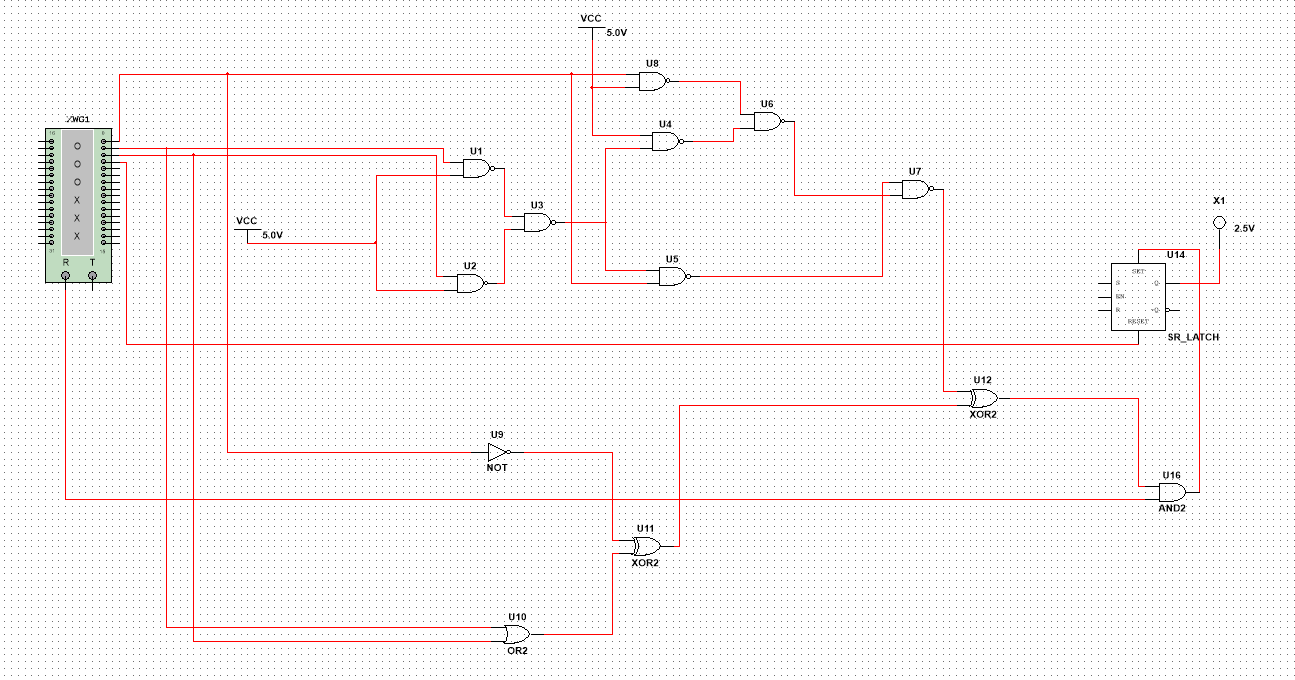
\includegraphics[width=\textwidth]{1ap}
\caption{Górna część układu to układ faktyczny, dolna część - układ testujący. Jeżeli w którymkolwiek momencie wykryta zostanie rozbieżność, przerzutnik po prawej "zapamięta" ten fakt.}
\end{figure}
Moduł XWG1 został zaprogramowany aby sprawdzał wszystkie możliwe konbinacje wartości A,B,C.
\subsection{Wnioski}
\paragraph{Kompletność NAND}
Należy zauważyyć, że bramka NAND jest wystarczająca to utworzenia pełnego systemu logicznego. Tj, dowolną skończoną funkcję logiczną można fizycznie zaimplementować za pomocą skończonej ilości bramek NAND. 
\paragraph{Przykładowe zastosowanie}
Układ może być wykorzystany do stworzenia systemu oświetlenia w części wspólnej składu w akademiku. (zmodyfikowany wyłącznik schodowy). Sygnał A odpowiadałby stanowi włącznika przy wejściu do składu, sygnały B i C - przy wejściu do pokojów.
\newpage
\section{Zadanie 1b}
\subsection{Treść zadania}
\paragraph{}
Rozważmy pomieszczenie w którym znajdują się: drzwi wejściowe i dwa okna (wszystko wyposażone w czujniki stanu zamknięcia). Poza tym znajduje się tam: czujnik ruchu, syrena alarmowa (może być reprezentowana wskaźnikiem LED), dwa przyciski: uzbrojenia i rozbrojenia alarmu, dwa wskaźniki LED: alarm uzbrojony i alarm wyłączony, LEDowy czerwony sygnalizator problemu załączenia alarmu.
\paragraph{}
Alarm można uzbroić dedykowanym przyciskiem tylko wtedy, gdy w pomieszczeniu nie wykryto ruchu, a drzwi i okna są skutecznie zamknięte. Wówczas powinna zaświecić się kontrolka uzbrojenia alarmu. Jeśli warunki te nie są spełnione, zaświeca się czerwony sygnalizator problemu, a alarm pozostaje rozbrojony, co ciągle wówczas sygnalizuje stosowny wskaźnik LED.
\paragraph{}
Poprawne uzbrojenie alarmu powoduje zgaszenie się wskaźnika rozbrojenia alarmu i sygnalizatora problemu (jeśli jest zaświecony) oraz powoduje zaświecenie się wskaźnika uzbrojenia alarmu.
\paragraph{}
Alarm uruchamia się, gdy system alarmowy jest uzbrojony i wykryty jest ruch lub sygnalizowane jest otwarcie: drzwi lub któregoś z okien.
\paragraph{}
W oparciu o dowolne bramki logiczne, przełączniki i wskaźniki LED, proszę zaprojektować, zminimalizować, zbudować i przetestować układ realizujący funkcję opisanego wyżej systemu alarmowego. Rolę czujników mogą tutaj pełnić dowolne (dostępne w Multisimie) źródła sygnału cyfrowego.
\subsection{Rozwiązanie teoretyczne}
\paragraph{Oznaczenia}
Przyjmijmy następujące oznaczenia sygnałów: \\
$A_{1} \dots A_{4}$ jako sygnały czujników, \\
B jako przycisk uzbrojenia, \\
C jako przycisk rozbrojenia, \\
D jako poprzedni stan odpowiedniego sygnału, \\
E jako sygnalizator problemu, \\
F jako stan uzbrojenia alarmu.
\subsubsection{Łączenie czujników}
Zauważmy, że z perspektywy alarmu, dowolne naruszenie czujników jest traktowane identycznie - nie interesuje nas to, czy otwarte są drzwi czy okna, w obu przypadkach można się dostać do pomieszczenia. Możemy więc utworzyć sygnał łączny czujników, dalej oznaczony jako $A$.
Mamy totaj do czynienia z następującą tabelą prawdy: \\
\begin{center}
\begin{tabular}{c c}
Sygnały czujników $A_{1} \dots A_{4}$ & Sygnał A \\
\hline
0000 & 0 \\
Dowolny inny & 1
\end{tabular}
\end{center}
Z praw logiki można bespośrednio wyprowadzić $A = A_{1} + A_{2} + A_{3} + A_{4}$.
\subsection{Wyprowadzenie wzorów}
\subsubsection{Sygnalizator błędu}
\begin{figure}[H]
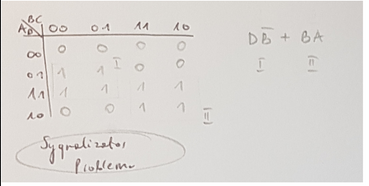
\includegraphics[width=0.7\textwidth]{error}
\caption{Tabela Karnaugh odpowiadająca sygnałowi błędu.}
\end{figure}
\subsubsection{Stan uzbrojenia}
\begin{figure}[H]
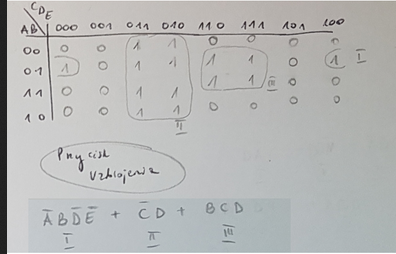
\includegraphics[width=0.7\textwidth]{alarm}
\caption{Tabela Karnaugh odpowiadająca stanowi uzbrojenia.}
\end{figure}
\subsubsection{Syrena alarmowa}
\begin{figure}[H]
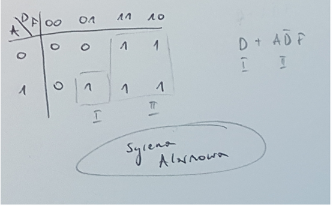
\includegraphics[width=0.7\textwidth]{syrena}
\caption{Tabela Karnaugh odpowiadająca syrenie alarmowej.}
\end{figure}

\subsection{Implementacja układu 1b w programie Multisim}
\begin{figure}[H]
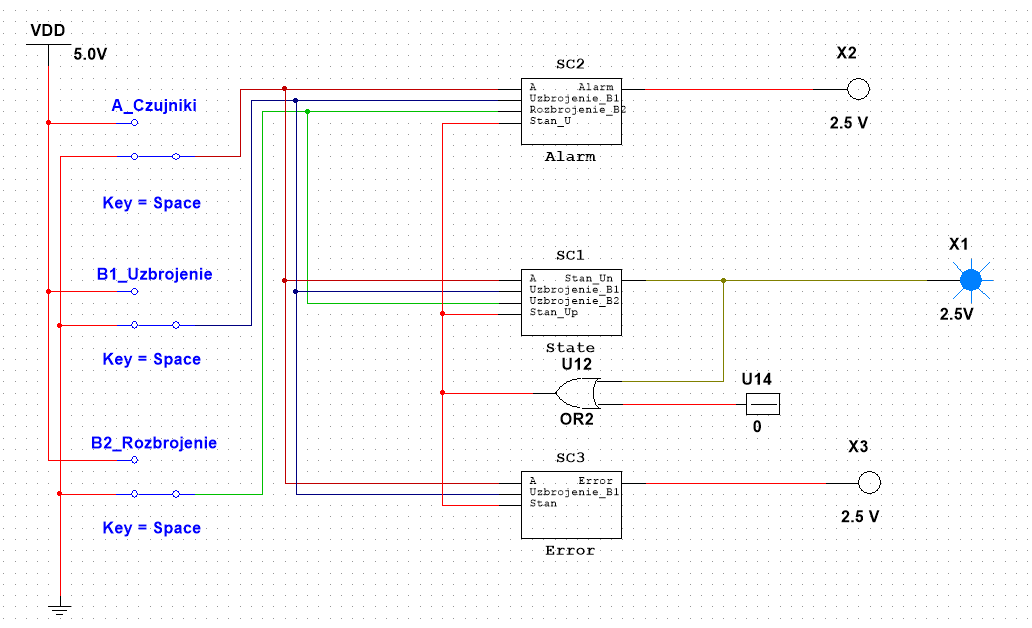
\includegraphics[width=0.7\textwidth]{fullMS}
\caption{Pełnny układ, zaimplementowany w programie Multisim. Podprojekty S1-S3 przedstawione poniżej.}
\end{figure}
\begin{figure}[H]
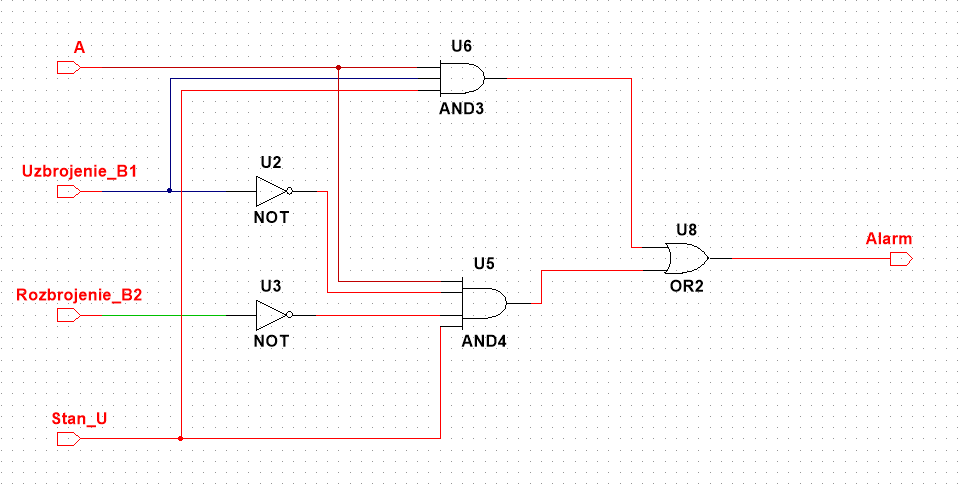
\includegraphics[width=0.7\textwidth]{alarmMS}
\caption{Implementacja sygnału uzbrojenia/rozbrojenia alarmu.}
\end{figure}
\begin{figure}[H]
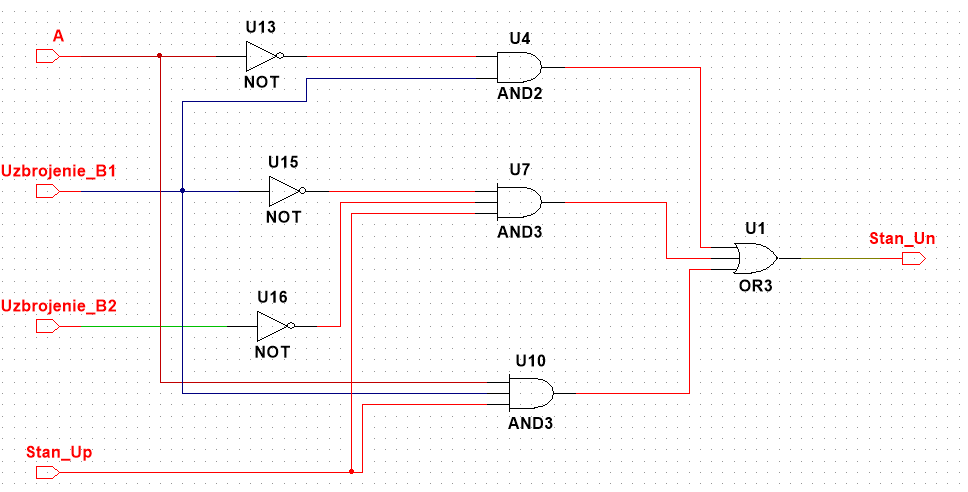
\includegraphics[width=0.7\textwidth]{syrenaMS}
\caption{Implemetacja sygnału syreny alarmowej}
\end{figure}
\begin{figure}[H]
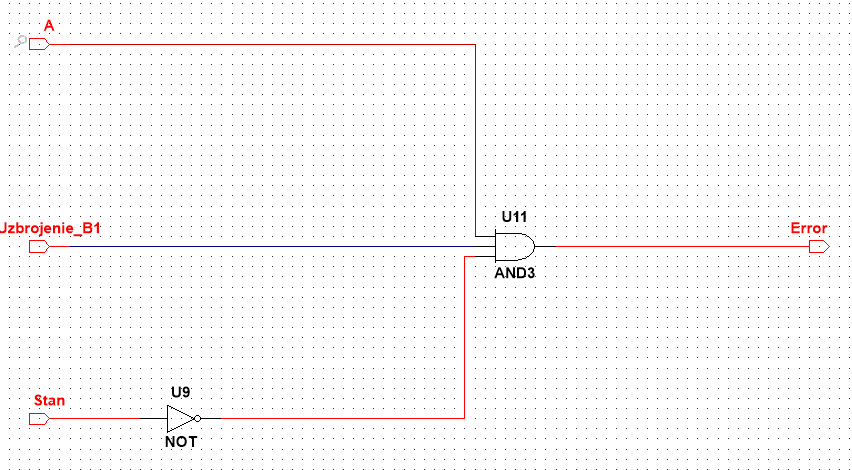
\includegraphics[width=0.7\textwidth]{errorMS}
\caption{Implementacja sygnału niepoprawnego uzbrojenia.}
\end{figure}
\begin{figure}[H]
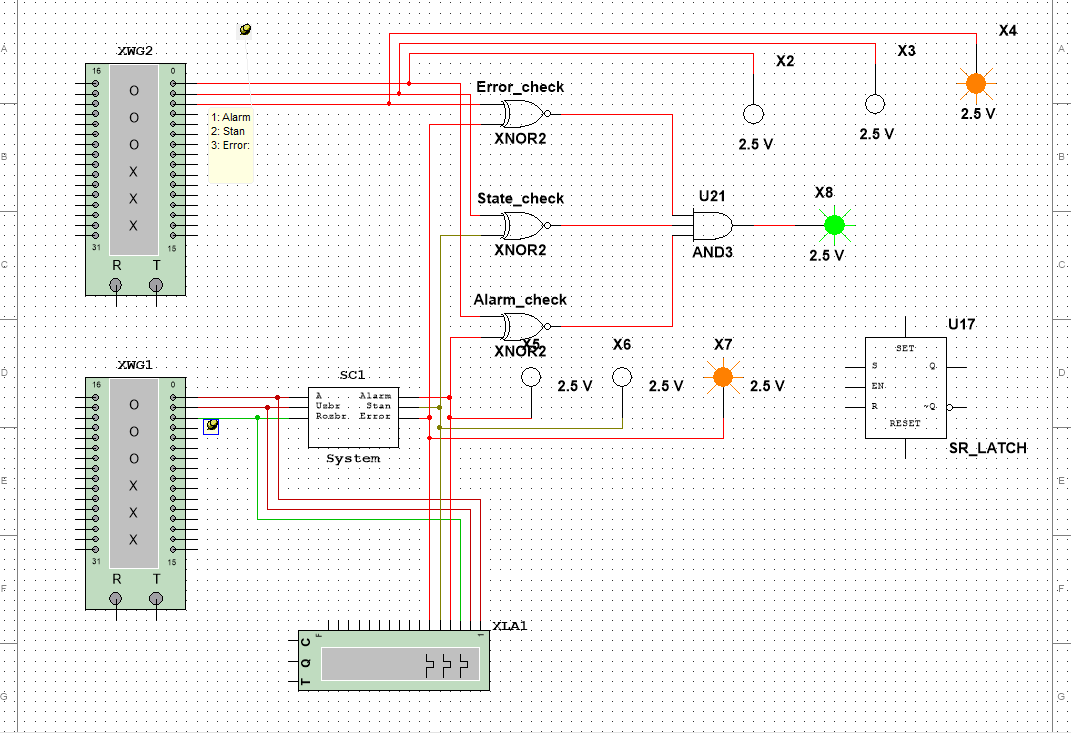
\includegraphics[width=0.7\textwidth]{testerMS}
\caption{Układ testujący nasz projekt (SC1). Górne lamki LED generują oczekiwany rezultat, dolne - rzeczywisty.}
\end{figure}


\subsection{Wnioski}
\paragraph{Prostota a praktyka}
Korzystając tylko z podstawowej wiedzy na temat bramek logicznych, jesteśmy w stanie zaprojektować układ stosowalny w życiu codziennym. Co więcej, mamy niemalże gwarancję że układ nasz będzie szybszy niż jakiekolwiek implementacje oparte o programowanie "klasycznego" procesora.
\end{document}